\documentclass[main.tex]{subfiles}

% Document
\begin{document}

\chapter{Simulating a double pendulum}

\section{Introduction}

In Part 2, we learned how to setup and run simulations, and how changing the integrator and step-size affected the accuracy of our results.  
In this section, we'll start simulating a more challenging system, where we don't necessarily know what answer to expect.  
%Three independent problems are outlined below.  
%Each problem has a number of extensions and possible routes to explore.  
%Feel free to concentrate on one problem, try a little bit from all of them, or come up with new questions to explore.  
%As long as we can figure out how to write down the derivative functions for the model you're interested in, there's a good chance we can simulate it using the tools we've developed!

%3.2 Orbital mechanics
%
%1 body equation
%Multiple bodies in COM frame
%Stability region for moon in R3BP
%Planet stability around binary star
%
%3.3 Projectile motion
%
%Normal motion in vacuum
%Add quadratic air resistance
%Optimize over angle
%
\section{Governing equations}

\begin{figure}
\centering
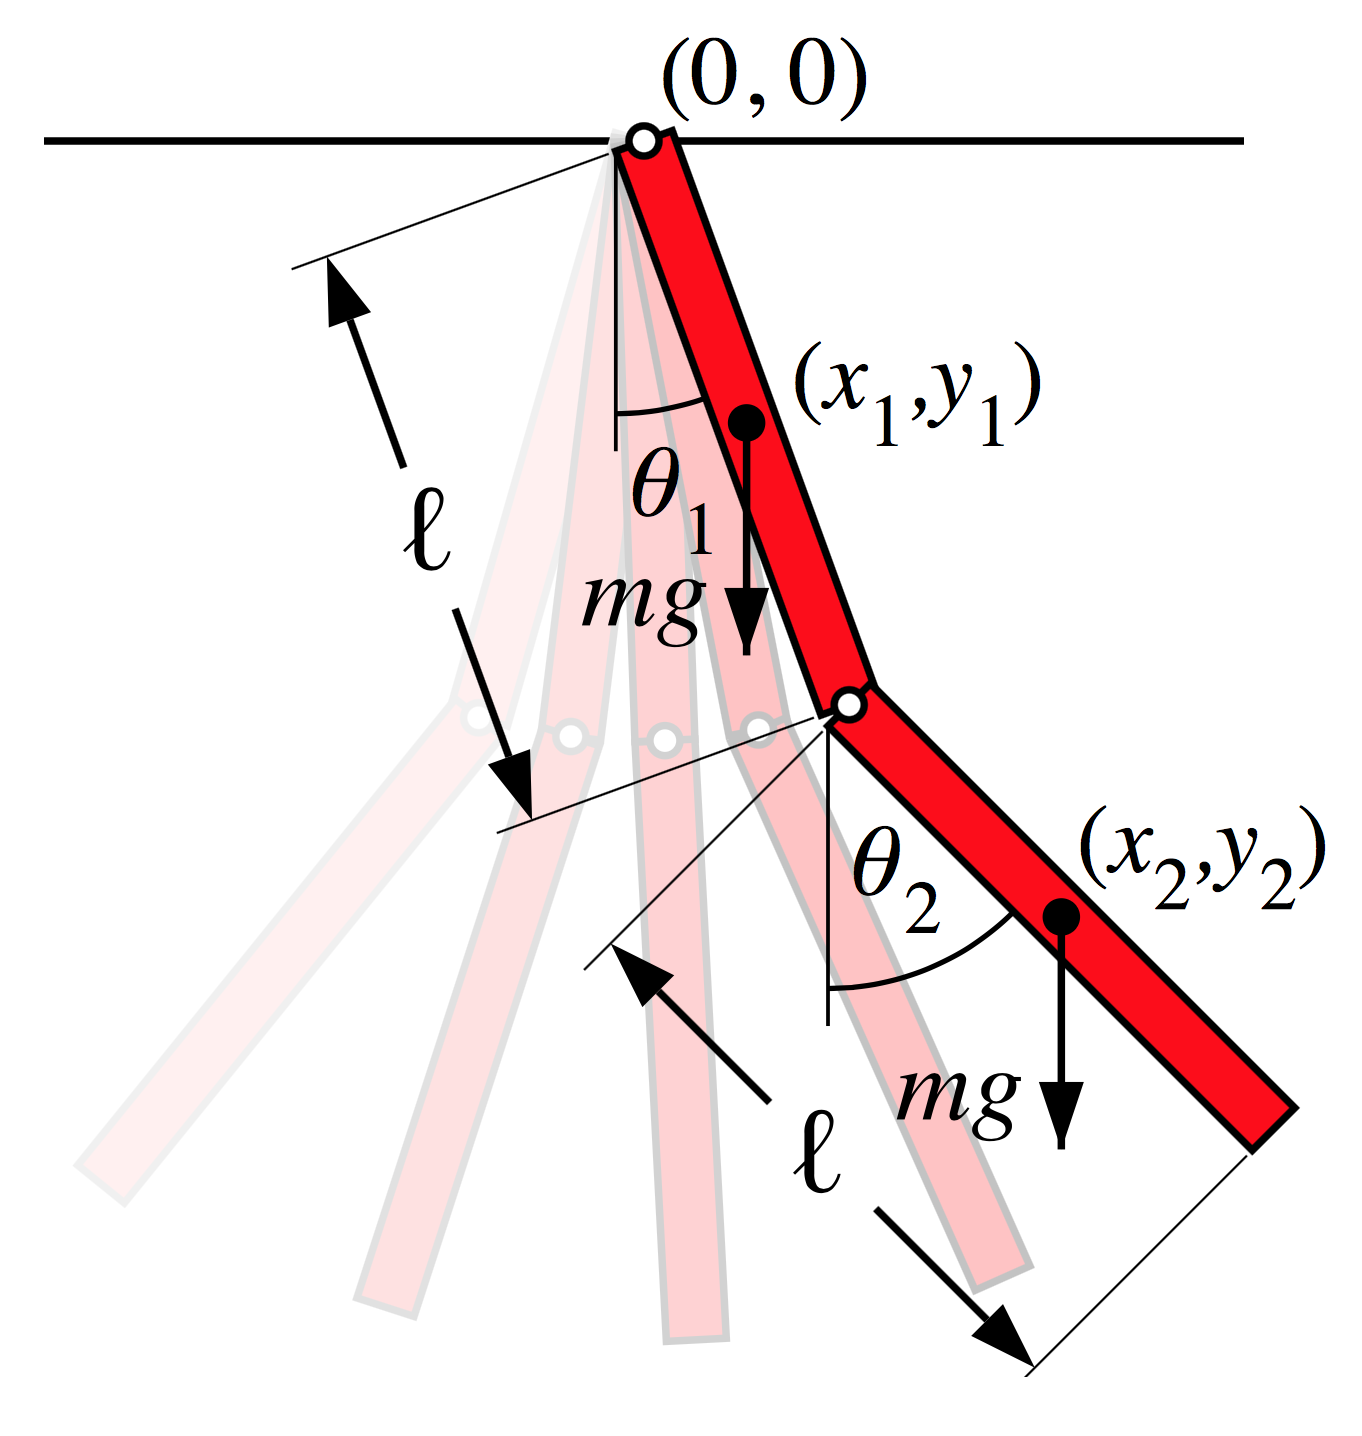
\includegraphics[width=0.4\textwidth]{images/pendulum}
\caption{Double pendulum (Wikipedia)}
\end{figure}

A double pendulum is a pendulum with an intermediate hinge point along its length (see image).  
The dynamics of a single pendulum are relatively simple and predictable, but a double pendulum is surprisingly different.

For simplicity, we'll consider a double pendulum consisting of two arms each of length $l$ and mass $m$.  
We could track the $x$ and $y$ position of the center of each pendulum, but it turns out to be easier to write down the equation for the angle $\theta$ that each pendulum makes relative to vertical.

Using Newton's laws, we can derive equations for the rotational acceleration of each pendulum under gravity.  
The algebra to write out all the terms, though, becomes very complicated, so instead of deriving the equations, we will just state them:

\begin{align}
    \dot{\theta}_1 &= \frac{6}{m l^2} \frac{2 p_1 - 3 p_2 \cos(\theta_1-\theta_2)}{16 - 9 \cos^2(\theta_1-\theta_2)} \\
    \dot{\theta}_2 &= \frac{6}{m l^2} \frac{8 p_2 - 3 p_1 \cos(\theta_1-\theta_2)}{16 - 9 \cos^2(\theta_1-\theta_2)} \\
    \dot{p}_1 &= -\frac{1}{2} m l^2 [3 \frac{g}{l} \sin \theta_1 + \dot{\theta}_1 \dot{\theta}_2 \sin(\theta_1-\theta_2)] \\
    \dot{p}_2 &= -\frac{1}{2} m l^2 [\frac{g}{l} \sin \theta_2 - \dot{\theta}_1 \dot{\theta}_2 \sin(\theta_1-\theta_2)] \\
\end{align}

Here $\theta_1$ and $\theta_2$ are the angles of the first and second arms relative to vertical, and $p_1$ and $p_2$ are the momenta of the arms.

Task: 
Write a Python function, matching the interface specified in Task 3, that returns the time-derivative system for the motion of a double pendulum.  
Let $U = [\theta_1, \theta_2, p_1, p_2]$ and set $g=9.8$, $m=1$, and $l=1$.

\section{Running a simulation}

For our initial conditions let's start by taking the pendulum to be stationary and angled at 45 degrees, i.e. $A = [\frac{\pi}{4}, \frac{\pi}{4}, 0, 0]$.

Task 9: 
Simulate the double pendulum to a final time $T=10$ using the Runge Kutta integrator.  
Run the simulation and use the first and second columns of $U$, which are $\theta_1$ and $\theta_2$, to compute positions of the ends of the two arms: $x_1$, $y_1$, $x_2$, $y_2$.  
Then plot the trajectory using the following code:

\begin{python}
t, U = simulate(U0, F, midpoint, T, h)
x1 = np.sin(U[:,0])
y1 = -np.cos(U[:,0])
x2 = x1 + np.sin(U[:,1])
y2 = y1 - np.cos(U[:,1])

plt.figure(figsize=(10,6))
plt.plot(0, 0, '.k')
plt.plot(x1, y1, '-b')
plt.plot(x2, y2, '-r')
plt.axis('equal')
plt.xlabel('x')
plt.ylabel('y')
\end{python}
Task 10: Make a video of your simulation using the following code:

\begin{python}
from matplotlib import animation
plt.ioff()
fig = plt.figure(figsize=(10,6))
line1, = plt.plot(x1, y1, '.-k', zorder=1, lw=3, ms=12)
line2, = plt.plot(x2, y2, '.-k', zorder=1, lw=3, ms=12)
line3, = plt.plot(0, 0, '-b', alpha=0.5, zorder=0)
line4, = plt.plot(0, 0, '-r', alpha=0.5, zorder=0)
title = plt.title('t = %.2f' %t[0])
plt.axis('equal')
plt.xlabel('x')
plt.ylabel('y')

fps = 50
dpi = 120
drag = int(0.25 / h)
N = int(T * fps)
skip = int(len(U) / N)
def animate(i):
    j = i*skip
    line1.set_data([0, x1[j]], [0, y1[j]])
    line2.set_data([x1[j], x2[j]], [y1[j], y2[j]])
    line3.set_data(x1[max(0,j-drag):j], y1[max(0,j-drag):j])
    line4.set_data(x2[max(0,j-drag):j], y2[max(0,j-drag):j])
    title.set_text('t = %.2f' %t[j])
    if i % 50 == 0:
        print('%i / %i' %(i, N), end='\r')
    return (line1, line2)

anim = animation.FuncAnimation(fig, animate, frames=N,
                               blit=True, repeat=False)
anim.save('./pendulum.mp4', dpi=dpi, fps=fps)
print('Finished    ')
plt.close()
plt.ion()
\end{python}

\end{document}
